%%% LaTeX Template: Article/Thesis/etc. with colored headings and special fonts
%%%
%%% Source: http://www.howtotex.com/
%%% Feel free to distribute this template, but please keep to referal to http://www.howtotex.com/ here.
%%% February 2011
%%%
%%% Modified Oct 2021 by CDM

%%%  Preamble
\documentclass[11pt,letterpaper]{article}
\usepackage[margin=1.0in]{geometry}
\usepackage[T1]{fontenc}
\usepackage[bitstream-charter]{mathdesign}
\usepackage[latin1]{inputenc}					
\usepackage{amsmath}						
\usepackage{xcolor}
\usepackage{cite}
\usepackage{hyphenat}
\usepackage{graphicx}
\usepackage{float}
\usepackage{subfigure}
\usepackage{sectsty}
\usepackage[compact]{titlesec} 
\usepackage[tablegrid]{vhistory}
\allsectionsfont{\color{accentcolor}\scshape\selectfont}

%%% Definitions
\definecolor{accentcolor}{rgb}{0.0,0.0,0.5} 
\newcommand{\teamname}{Team Mercury}
\newcommand{\productname}{ARGOOSE-Counter Drone Tracking}
\newcommand{\coursename}{CSE 4316: Senior Design I}
\newcommand{\semester}{Fall 2022}
\newcommand{\docname}{System Requirements Specification}
\newcommand{\department}{Department of Computer Science \& Engineering}
\newcommand{\university}{The University of Texas at Arlington}
\newcommand{\authors}{James Grumbles \\ Nirdesh Sakh \\ Augustine Nguyen \\ Sanyogita Piya \\ Mahin Roddur}

%%% Headers and footers
\usepackage{fancyhdr}
	\pagestyle{fancy}						% Enabling the custom headers/footers
\usepackage{lastpage}	
	% Header (empty)
	\lhead{}
	\chead{}
	\rhead{}
	% Footer
	\lfoot{\footnotesize \teamname \ - \semester}
	\cfoot{}
	\rfoot{\footnotesize page \thepage\ of \pageref{LastPage}}	% "Page 1 of 2"
	\renewcommand{\headrulewidth}{0.0pt}
	\renewcommand{\footrulewidth}{0.4pt}

%%% Change the abstract environment
\usepackage[runin]{abstract}			% runin option for a run-in title
%\setlength\absleftindent{30pt}			% left margin
%\setlength\absrightindent{30pt}		% right margin
\abslabeldelim{\quad}	
\setlength{\abstitleskip}{-10pt}
\renewcommand{\abstractname}{}
\renewcommand{\abstracttextfont}{\color{accentcolor} \small \slshape}	% slanted text

%%% Start of the document
\begin{document}

%%% Cover sheet
{\centering \huge \color{accentcolor} \sc \textbf{\department \\ \university} \par}
\vspace{1 in}
{\centering \huge \color{accentcolor} \sc \textbf{\docname \\ \coursename \\ \semester} \par}
\vspace{0.5 in}
\begin{figure}[h!]
	\centering
   	
\includegraphics[width=0.60\textwidth]{images/Logo (1).PNG}
\end{figure}
\vspace{0.5 in}
{\centering \huge \color{accentcolor} \sc \textbf{\teamname \\ \productname} \par}
\vspace{0.5 in}
{\centering \large \sc \textbf{\authors} \par}
\newpage


%\vspace{1 in}
%\centerline{January 13th, 2012}
%\newpage

%%% Revision History
\begin{versionhistory}
  	\vhEntry{0.1}{9.23.2022}{AN}{document creation}
  	\vhEntry{0.2}{10.23.2022}{AN|JG|SP|NS|MR}{complete draft}
\end{versionhistory}
\newpage

%%% Table of contents
\setcounter{tocdepth}{3}
\tableofcontents
\newpage

%%% List of figures and tables (optional)
\listoffigures
%\listoftables
\newpage

\section{Product Concept}
This section provides a high-level statement of your product concept - what it is intended to do and how it is intended to be used. Include in this header paragraph, a brief synopsis of what is described here. For example, this header paragraph might say something like: "This section describes the purpose, use and intended user audience for the X product. X is a system that performs Y. Users of X will be able to Z..."

\subsection{Purpose and Use}
This is where you describe in a brief, yet clear and concise, manner what your product should do and how you expect it should be used.

\subsection{Intended Audience}
This is where you describe the intended audience(s) of your product. If this product were to be made available publicly or commercially, who would purchase or use it? Is the product designed for a particular customer, or an overall class of customers? Is it intended for general use, or is it a specific component of a more complex system?

\begin{figure}[h!]
	\centering
   	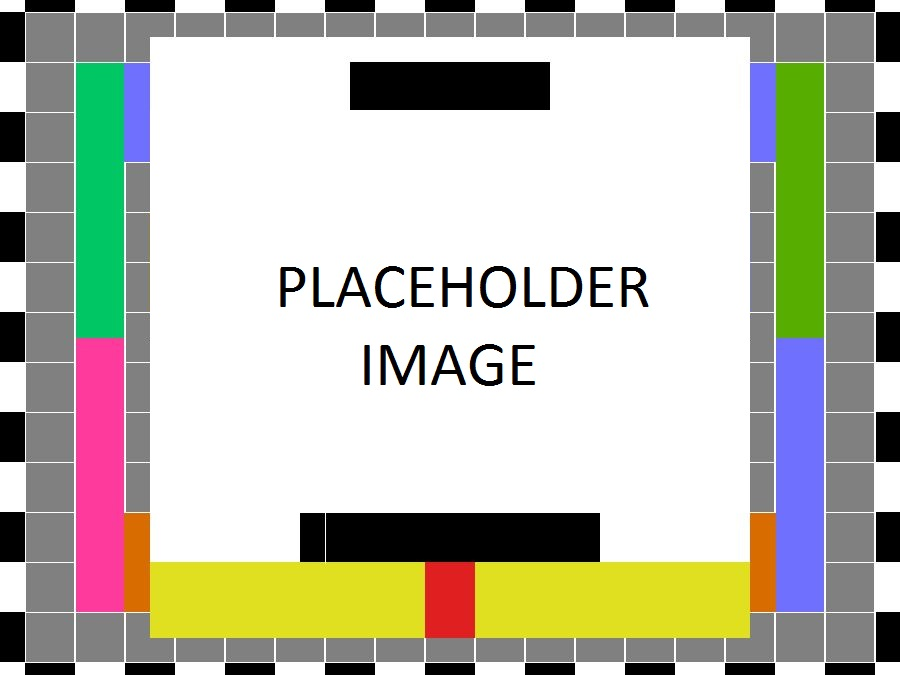
\includegraphics[width=0.60\textwidth]{images/test_image}
    \caption{X conceptual drawing}
\end{figure}

\newpage
\section{Product Description}
This section provides a description of your product and defines it's primary features and functions. The purpose is to give the document reader/reviewer enough information about the product to allow them to easily follow the specification of requirements found in the remainder of the document. Your header for this section should introduce the section with a brief statement such as: "This section provides the reader with an overview of X. The primary operational aspects of the product, from the perspective of end users, maintainers and administrators, are defined here. The key features and functions found in the product, as well as critical user interactions and user interfaces are described in detail." Using words, and pictures or graphics where possible, specify the following:

\subsection{Features \& Functions}
What the product does and does not do. Specify in words what it looks like, referring to a conceptual diagram/graphic (Figure X).  Define the principle parts/components of the product. Specify the elements in the diagram/graphic that are part(s) of this product as well as any associated external elements (e.g., the Internet, an external web server, a GPS satellite, etc.)

\subsection{External Inputs \& Outputs}
Describe critical external data flows. What does your product require/expect to receive from end users or external systems (inputs), and what is expected to be created by your product for consumption by end users or external systems (outputs)? In other words, specify here all data/information to flow into and out of your systems. A table works best here, with rows for each critical data element, and columns for name, description and use.

\subsection{Product Interfaces}
Specify what all operational (visible) interfaces look like to your end-user, administrator, maintainer, etc. Show sample/mocked-up screen shots, graphics of buttons, panels, etc. Refer to the critical external inputs and outputs described in the paragraph above.

\newpage
\section{Customer Requirements}
\subsection{The system shall show the current location of the device placed}
\subsubsection{Description}
The system will track the current location using maps and display it through API.
\subsubsection{Source}
Customer Requirement
\subsubsection{Constraints}
There is no realistic constraint for this requirement. Our web app should accurately display the location of the tracking devices placed.
\subsubsection{Standards}
There are no intrinsic standards to meet this requirement.
\subsubsection{Priority}
This is a critical priority for the project.

\subsection{The system shall notify the customer if a drone passes by}
\subsubsection{Description}
The system will give a message alert to the customer and the point at which the drone signal was captured if a drone is detected in the radius of the device.
\subsubsection{Source}
Customer Requirement
\subsubsection{Constraints}
The device should be turned on and ready to process the auditory and RF.
\subsubsection{Standards}
There are no intrinsic standards to meet this requirement.
\subsubsection{Priority}
This is a high level Priority for the project.

\subsection{The system shall show the path in the web application in which the drone travels}
\subsubsection{Description}
The system marks the path on the maps along which the drone passes by in the radius of the device.
\subsubsection{Source}
Customer Requirement
\subsubsection{Constraints}
The path will only be visible temporarily.
\subsubsection{Standards}
There are no intrinsic standards to meet this requirement.
\subsubsection{Priority}
This is a low level Priority for the project.

\subsection{The system shall categorize the data input from the sensors into potential drones and non drone objects.}
\subsubsection{Description}
The system will use machine learning concepts for this categorization.
\subsubsection{Source}
Customer Requirement
\subsubsection{Constraints}
The sensors should be placed in an open area without any significant disturbances.
\subsubsection{Standards}
There are no intrinsic standards to meet this requirement.
\subsubsection{Priority}
This is a critical level Priority for the project.

\subsection{UI Requiremetn}
\subsubsection{Description}
The user will have to register and login to the system in order to use it. The registration system will be delivered to correctly identify the user logs. The passwords shall be encrypted using SSL.
\subsubsection{Source}
Customer Requirement
\subsubsection{Constraints}
The password will have standard constraints: 7 letters, one capital letter, one small letter, one number and one special character.
\subsubsection{Standards}
Registration username will be email address that will need to be verified
\subsubsection{Priority}
This is a low level Priority for the project.

\newpage
\section{Packaging Requirements}
Include a header paragraph here. Packaging requirements are those requirements that identify how the delivered product will be packaged for delivery to the end-user; or how it will "look" when finished and delivered. For example, you might specify that the software required for operation will be pre-loaded on the hard drive, delivered on CD/DVD, or available via download. Software might be customer installable, or not, etc. Hardware components could be all in a single package, provided as a "bag of parts" to be assembled/installed by the user, painted a certain color, logos affixed, etc. Care should be taken not to duplicate requirements found in other sections of this document.

\subsection{The delivered product will be in form of a ground based sensor device and a web application.}
\subsubsection{Description}
The ground based sensor device shall capture the acoustic signals and provide it to the system and the web based application would show the results of the inputs
\subsubsection{Source}
Sanyogita Piya
\subsubsection{Constraints}
N/A
\subsubsection{Standards}
In order to run the web application, the user should have access to internet.
\subsubsection{Priority}
Critical

\subsection{The ground based drone detection sensor system shall weigh less than 50 lbs}
\subsubsection{Description}
The only hardware system that is presented to the customer is the ground based sensor system hence there is a weight limit associated to it.
\subsubsection{Source}
Sanyogita Piya
\subsubsection{Constraints}
N/A
\subsubsection{Standards}
N/A
\subsubsection{Priority}
High


\subsection{The integration setup of the system shall be simple and easy to follow}
\subsubsection{Description}
The user manual shall be provided to the customer which would have a step by step set up guideline to start the system.
\subsubsection{Source}
Sanyogita Piya
\subsubsection{Constraints}
N/A
\subsubsection{Standards}
N/A
\subsubsection{Priority}
High

\newpage
\section{Performance Requirements}
Include a header paragraph specific to your product here. Performance requirements address items such as: how fast specific critical operations must complete; how long it takes to start/stop activities; how long the battery must last; maximum time it must take to set up; etc.

\subsection{System will maintain a false positive rate below 15 percent}
\subsubsection{Description}
When passively detecting drones, the system will not identify incorrectly by pinging the web interface more than 15 percent of the time. False positives will consist of any detection alert that identifies an item in space that is not a drone or drone similar object.
\subsubsection{Source}
Performance Requirement
\subsubsection{Constraints}
Degraded performance due to weather effects may impact performance.
\subsubsection{Standards}
There are no intrinsic standards to meet this requirement.
\subsubsection{Priority}
This is a High priority requirement.

\subsection{System shall verify drones with acoustic detection with a subsystem backup}
\subsubsection{Description}
After detecting a drone utilizing it's primary acoustic system, the system will utilize a secondary detection system to verify it's possible drone detection. When both systems return a positive result, the web interface will be informed of a drone detected.
\subsubsection{Source}
Performance Requirement
\subsubsection{Constraints}
Degraded performance due to weather effects may impact performance.
\subsubsection{Standards}
There are no intrinsic standards to meet this requirement.
\subsubsection{Priority}
This is a Critical requirement.
\newpage
\section{Safety Requirements}
Detection system conforms to all applicable UTA standards and federal law

\subsection{Laboratory equipment lockout/tagout (LOTO) procedures}
\subsubsection{Description}
Any fabrication equipment provided used in the development of the project shall be used in accordance with OSHA standard LOTO procedures. Locks and tags are installed on all equipment items that present use hazards, and ONLY the course instructor or designated teaching assistants may remove a lock. All locks will be immediately replaced once the equipment is no longer in use.
\subsubsection{Source}
CSE Senior Design laboratory policy
\subsubsection{Constraints}
Equipment usage, due to lock removal policies, will be limited to availability of the course instructor and designed teaching assistants.
\subsubsection{Standards}
Occupational Safety and Health Standards 1910.147 - The control of hazardous energy (lockout/tagout).
\subsubsection{Priority}
Critical

\subsection{National Electric Code (NEC) wiring compliance}
\subsubsection{Description}
Any electrical wiring must be completed in compliance with all requirements specified in the National Electric Code. This includes wire runs, insulation, grounding, enclosures, over-current protection, and all other specifications.
\subsubsection{Source}
CSE Senior Design laboratory policy
\subsubsection{Constraints}
High voltage power sources, as defined in NFPA 70, will be avoided as much as possible in order to minimize potential hazards.
\subsubsection{Standards}
NFPA 70
\subsubsection{Priority}
Critical

\subsection{RIA robotic manipulator safety standards}
\subsubsection{Description}
Robotic manipulators, if used, will either housed in a compliant lockout cell with all required safety interlocks, or certified as a "collaborative" unit from the manufacturer.
\subsubsection{Source}
CSE Senior Design laboratory policy
\subsubsection{Constraints}
Collaborative robotic manipulators will be preferred over non-collaborative units in order to minimize potential hazards. Sourcing and use of any required safety interlock mechanisms will be the responsibility of the engineering team.
\subsubsection{Standards}
ANSI/RIA R15.06-2012 American National Standard for Industrial Robots and Robot Systems, RIA TR15.606-2016 Collaborative Robots
\subsubsection{Priority}
Critical

\subsection{UTA UAV Flying Guidelines}
\subsubsection{Description}
The project has to obey UTA's Guidelines on unmanned aircraft vehicles, so long as we are conducting under the school space.
\subsubsection{Source}
UTA Drone Policy
\subsubsection{Constraints}
UTA defines its safe fly zones and outlines its guidelines on how to conduct one's self when flying under UTA's jurisdiction.
\subsubsection{Standards}
CO-CS-PO-07 Unmanned Aircraft Systems Policy
\subsubsection{Priority}
Critical

\subsection{FAA UAV Flying Laws}
\subsubsection{Description}
The project must obey FAA laws involving unmanned aircraft vehicles
\subsubsection{Source}
Federal and State Drone Laws
\subsubsection{Constraints}
FAA descibes who is qualified to pilot, responsibilities of pilots, and pretty much any outlines every guideline on how to handle drones.
\subsubsection{Standards}
SMALL UNMANNED AIRCRAFT SYSTEMS (PART 107)
\subsubsection{Priority}
Critical
\newpage
\section{Security Requirements}
Include a header paragraph specific to your product here. In this section specify any requirements related to information security or privacy. This may include items such as encryption standards, data storage procedures, authentication, password strength, etc.
\subsection{Code base contained in repository shall remain private once product is finished}
\subsubsection{Description}
Code base is contained in git repository and will become private in terms of viewing and editing once the product is released.  For now, the product is able to be viewed publicly.  Only owner(s) and individuals appointed by the owner(s) may have access.
\subsubsection{Source}
Augustine Nguyen
\subsubsection{Constraints}
Private means no viewing or editing.  Access is given through the discretion of the owner(s).
\subsubsection{Standards}
N/A
\subsubsection{Priority}
Medium
\newpage
\section{Maintenance \& Support Requirements}
Include a header paragraph specific to your product here. Maintenance and support requirements address items specific to the ongoing maintenance and support of your product after delivery. Think of these requirements as if you were the ones who would be responsible for caring for customers/end user after the product is delivered in its final form and in use "in the field". What would you require to do this job? Specify items such as: where, how and who must be able to maintain the product to correct errors, hardware failures, etc.; required support/troubleshooting manuals/guides; availability/documentation of source code; related technical documentation that must be available for maintainers; specific/unique tools required for maintenance; specific software/environment required for maintenance; etc.

\subsection{Requirement Name}
\subsubsection{Description}
Detailed requirement description...
\subsubsection{Source}
Source
\subsubsection{Constraints}
Detailed description of applicable constraints...
\subsubsection{Standards}
List of applicable standards
\subsubsection{Priority}
Priority
\newpage
\section{Future Items}
Possible future implementations may, if possible, include advancements in the current system specifications. The system does not address historical data factors and may be included in future updates. As well as this, the ability to real time track, and also to track in real time multiple drones will not be included in the base model design. Altitude detection may, depending on time, be included but is restricted to a future implementation as it is a possible blocker for other core implementations at this time. Tertiary detection methods may also be added after initial system is completed and expandability is addressed.

\subsection{System will track multiple drones at one time}
\subsubsection{Description}
The system will be capable of selecting and actively tracking multiple drones it detects at any given time.
\subsubsection{Source}
Future Requirement
\subsubsection{Constraints}
Degraded performance due to weather effects may impact performance.
\subsubsection{Standards}
There are no intrinsic standards to meet this requirement.
\subsubsection{Priority}
This is a possible Future implementation.

\subsection{System will provide real time response to multiple drone scenarios}
\subsubsection{Description}
While actively tracking multiple drones, the system will provide close to real time data updates to be displayed.
\subsubsection{Source}
Future Requirement
\subsubsection{Constraints}
Degraded performance due to weather effects may impact performance.
\subsubsection{Standards}
There are no intrinsic standards to meet this requirement.
\subsubsection{Priority}
This is a possible Future implementation.

\subsection{The system shall be able to detect altitude of UAVs}
\subsubsection{Description}
On top of determining the top-down location of drones, the system should also be able to determine the height of where the drones are.  The technique for this has yet to be determined, but the output shall simply be a number and metric displayed somewhere on the user interface (e.g., 70 meters, 120 ft); more than likely, this feature will only be implemented for one drone at a time.
\subsubsection{Source}
Augustine Nguyen
\subsubsection{Constraints}
Altitude calculation will be for drones within a set area (yet to be determined), most definitely within the radius of the main detection system.  It will also be done for one drone at time.
\subsubsection{Standards}
N/A
\subsubsection{Priority}
Future

\subsection{The system shall send an email for the alert if a drone passes by the perimeter.}
\subsubsection{Description}
The user will have choice to select the medium of alert as email or text. Alerts are configurable and can also be sent to local law enforcement for a coordinated response.
\subsubsection{Source}
Sanyogita Piya
\subsubsection{Constraints}
N/A
\subsubsection{Standards}
N/A
\subsubsection{Priority}
Future

\subsection{Third Detection Layer: Computer vision implementation}
\subsubsection{Description}
If time and budget allows for it, detection through visual data stream can add another layer of drone detection verification. Although it seems unviable at the moment, a future implementation would add to the system's functionality.
\subsubsection{Source}
Mahin Roddur
\subsubsection{Constraints}
Budgetary and time constraints are the most apparent one here. 
\subsubsection{Standards}
N/A
\subsubsection{Priority}
Future

\subsection{The system shall store the history of drones detected}
\subsubsection{Description}
The system makes a log of time and the location of when a drone detected.
\subsubsection{Source}
This is a customer requirement.
\subsubsection{Constraints}
The history data will only be shown for the previous 7 days.
\subsubsection{Standards}
There are no intrinsic standards to meet this requirement.
\subsubsection{Priority}
Low Priority

\subsection{UI upgrade}
\subsubsection{Description}
The system should display the profile of the user with the option to change email address and change password. The system will have a profile database which stores the history of drone tracking, gives an option for the user to change their username and password.
\subsubsection{Source}
This is a customer requirement.
\subsubsection{Constraints}
The password will have standard constraints: 7 letters, one capital letter, one small letter, one number and one special character.
\subsubsection{Standards}
There are no intrinsic standards to meet this requirement.
\subsubsection{Priority}
Low Priority

\newpage

%%% References
\bibliographystyle{plain}
\bibliographystyle{reference/IEEEtran_custom}
\bibliography{reference/refs}{}

\end{document}